\documentclass[11pt]{beamer}
\usetheme{Warsaw}
\usepackage[utf8]{inputenc}
\usepackage[english]{babel}
\usepackage{amsmath}
\usepackage{amsfonts}
\usepackage{amssymb}
\usepackage{graphicx,wrapfig,lipsum}
\usepackage{multirow}



\author{Sascha Wernegger}
\title{Multimedia Data Formats}
%\setbeamercovered{transparent} 
%\setbeamertemplate{navigation symbols}{} 
%\logo{} 
%\institute{} 
%\date{} 
%\subject{} 

\newenvironment<>{varblock}[2][.9\textwidth]{%
  \setlength{\textwidth}{#1}
  \begin{actionenv}#3%
    \def\insertblocktitle{#2}%
    \par%
    \usebeamertemplate{block begin}}
  {\par%
    \usebeamertemplate{block end}%
  \end{actionenv}}
\begin{document}

\setcounter{tocdepth}{1}

\begin{frame}
\titlepage
\end{frame}

%\begin{frame}
%\tableofcontents
%\end{frame}

\section{Introduction}
	
\begin{frame}{Table of Contents}
        \tableofcontents[currentsection,currentsubsection]
\end{frame}

\begin{frame}{Content Based Image Retrieval}
\begin{block} {CBIR}
	\begin{itemize}
		\item \textbf{retrieval:} search images in large dataset
		\item \textbf{content based:} use image data of reference to find similar images
	\end{itemize}
\end{block}
\begin{block}{How to measure the influence of compression?}
	\begin{itemize}
		\item use retrieval system and calculate some performance measure for the results
		\item Use lossless compressed dataset and run retrieval system to calculate the performance
		\item Compress dataset to different and formats ratios and do the same
		\item interpret results
	\end{itemize}
\end{block}

\end{frame}

\begin{frame}{Software}
\begin{block}{VlBenchmark,VLFeat}
	\begin{itemize}
		\item feature extractors
		\item retrieval system
		\item performance measure
		\item dataset
	\end{itemize}
\end{block}
\begin{block}{OpenCV}
	\begin{itemize}
		\item feature extractors
	\end{itemize}
\end{block}
\begin{block}{ImageMagick,JXRLIB}
	\begin{itemize}
		\item compression
	\end{itemize}
\end{block}
\end{frame}


\section{Performance Evaluation}

\begin{frame}{Table of Contents}
        \tableofcontents[currentsection,currentsubsection]
\end{frame}
\subsection{Recall Precision}
\begin{frame}{Recall Precision}
	\begin{tabular}{ll}

		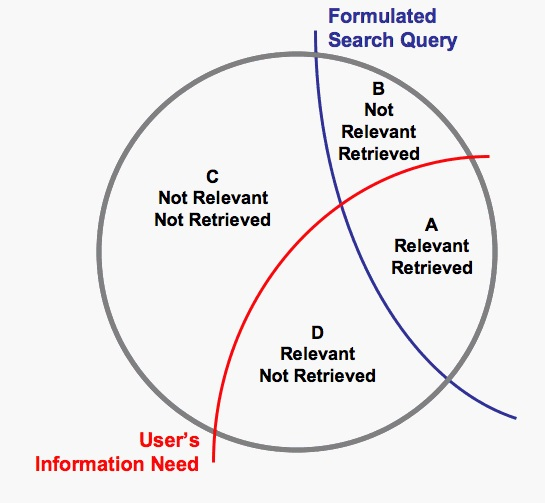
\includegraphics[width=0.5\textwidth]{img/RecallPrecision.jpg}
		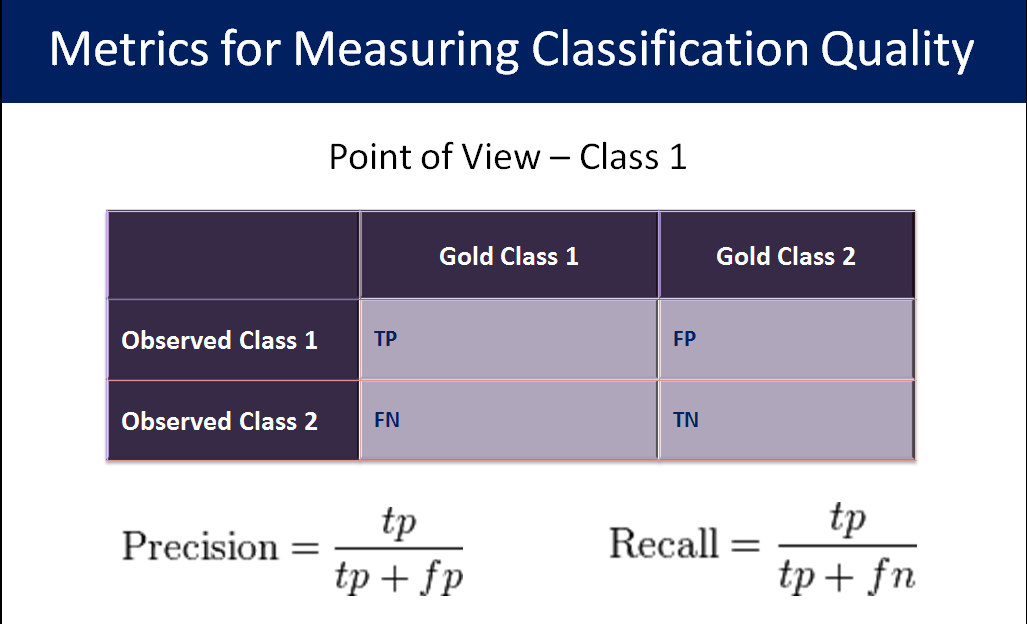
\includegraphics[width=0.5\textwidth]{img/precision_recall.png}

	\end{tabular}

\end{frame}

\begin{frame}{Recall Precision}

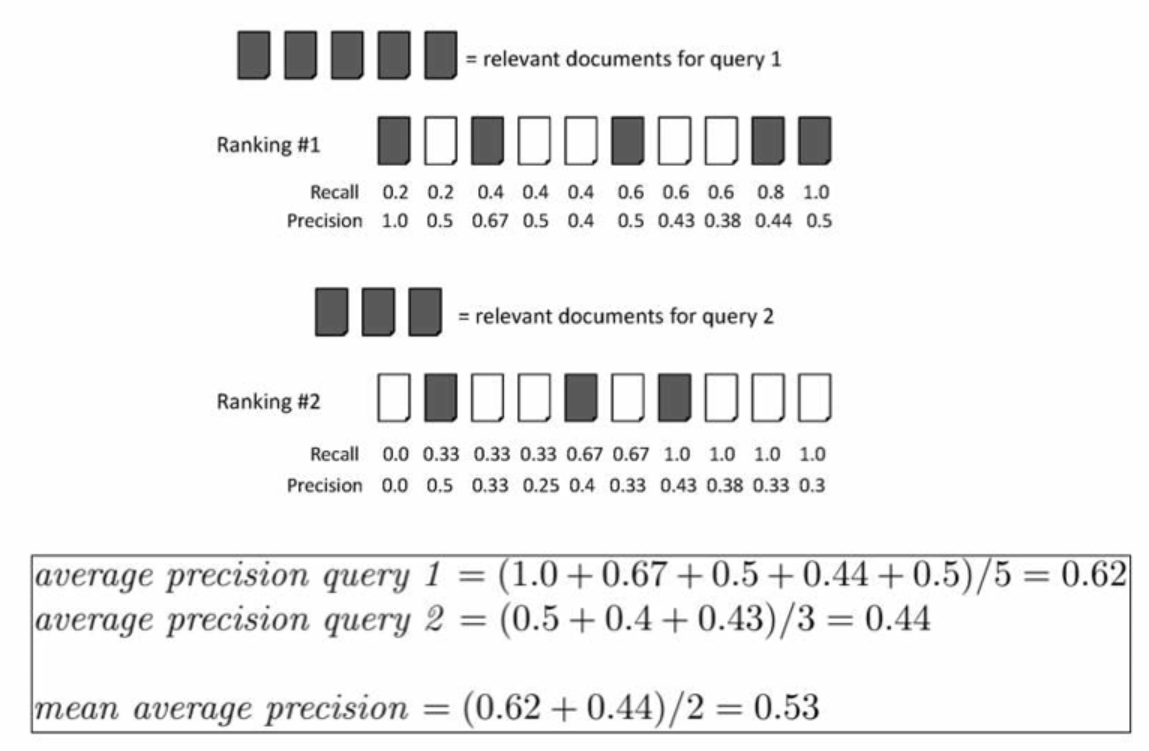
\includegraphics[width=0.9\textwidth]{img/map.png}

\end{frame}


\begin{frame}{Precision Recall Curves}
\begin{wrapfigure}{tr}{6.5cm}
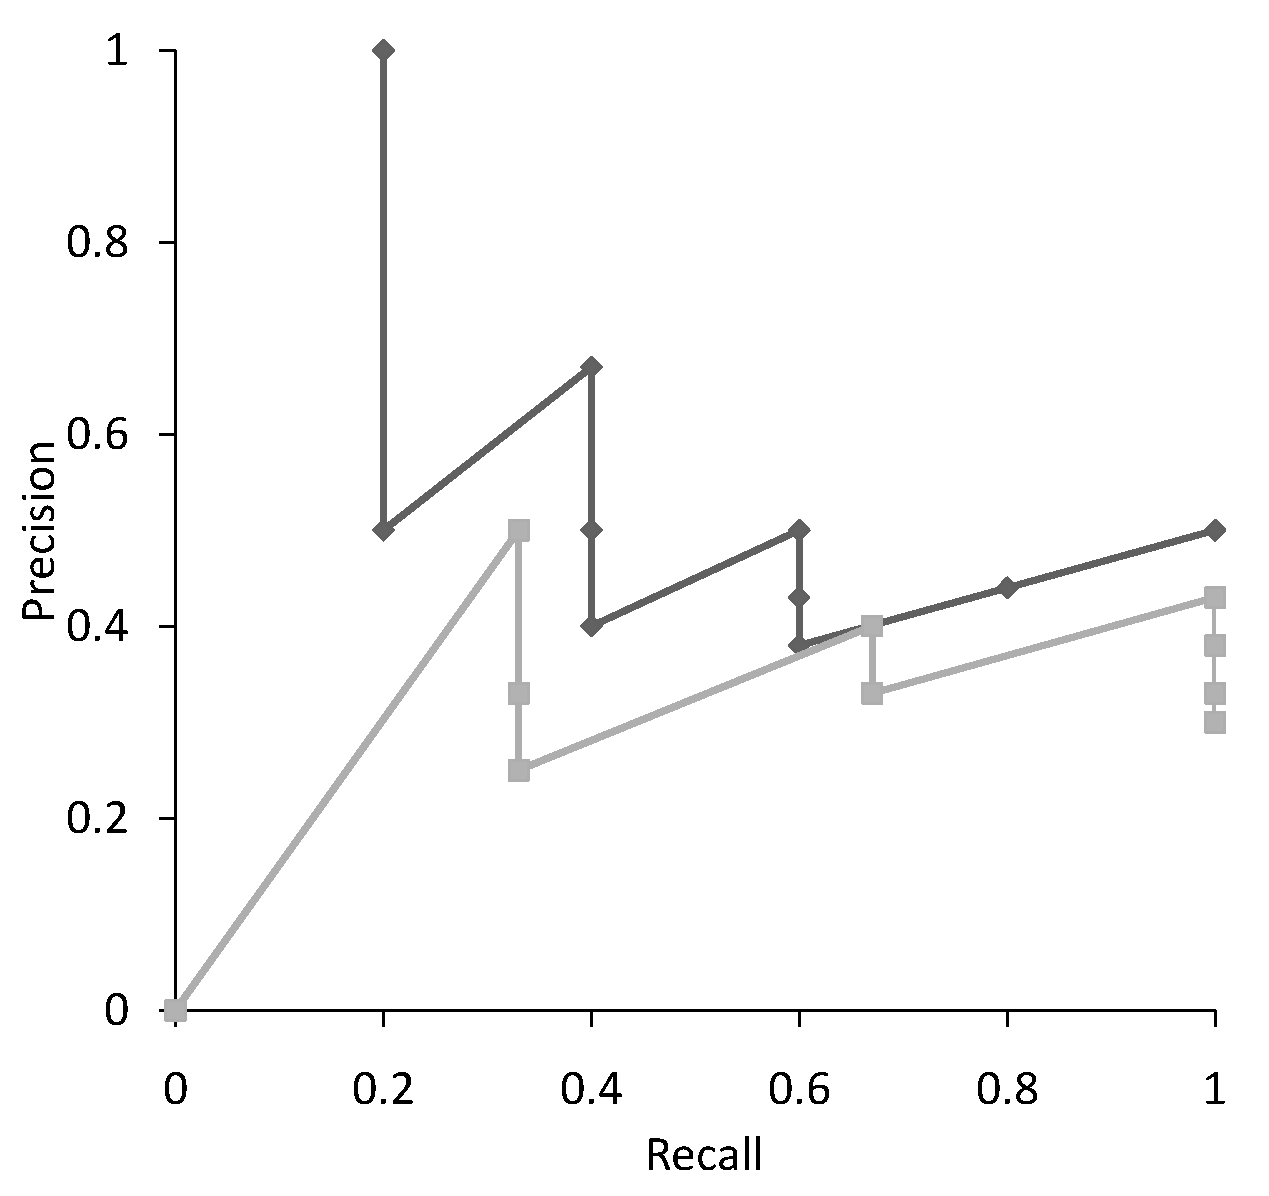
\includegraphics[width=5cm]{img/multi_prc.png}
\end{wrapfigure} 

To visualize precision and recall, we plot precision over recall.\\
If we have many queries, it is easier to interpret an averaged interpolated precision recall curve
\end{frame}

\begin{frame}{Interpolate PRC}
\begin{tabular}{ll}
\multirow{5}{*}{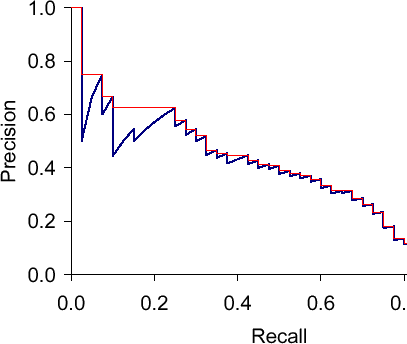
\includegraphics[width=0.45\textwidth]{img/prc.png} }
&Calculate precision at each\\
&recall level R as the\\
&maximum precision observed\\
&in any recall-precision point\\
&at a higher recall level
\end{tabular}
\end{frame}

\begin{frame}{Interpolate PRC}
\begin{wrapfigure}{tr}{6.5cm}
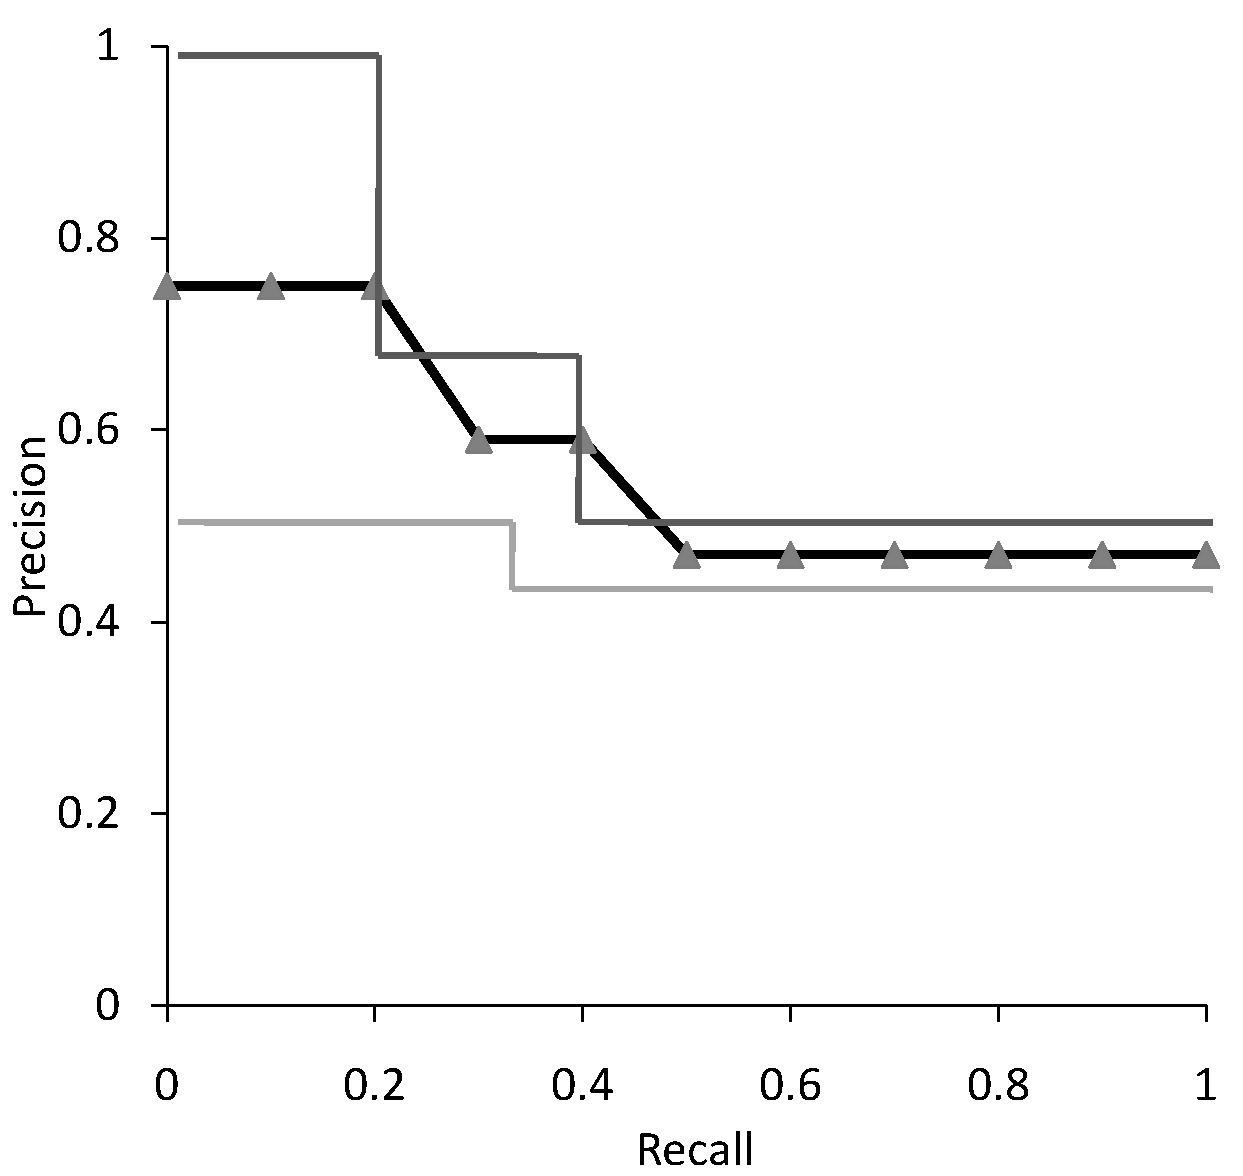
\includegraphics[width=5cm]{img/prc_average.png}
\end{wrapfigure} 
Calculate precision at each
recall level R as the
maximum precision observed
in any recall-precision point
at a higher recall level
\end{frame}

\subsection{Mean Average Precision}

\begin{frame}{Mean Average Precision}

\begin{wrapfigure}{l}{6.2cm}
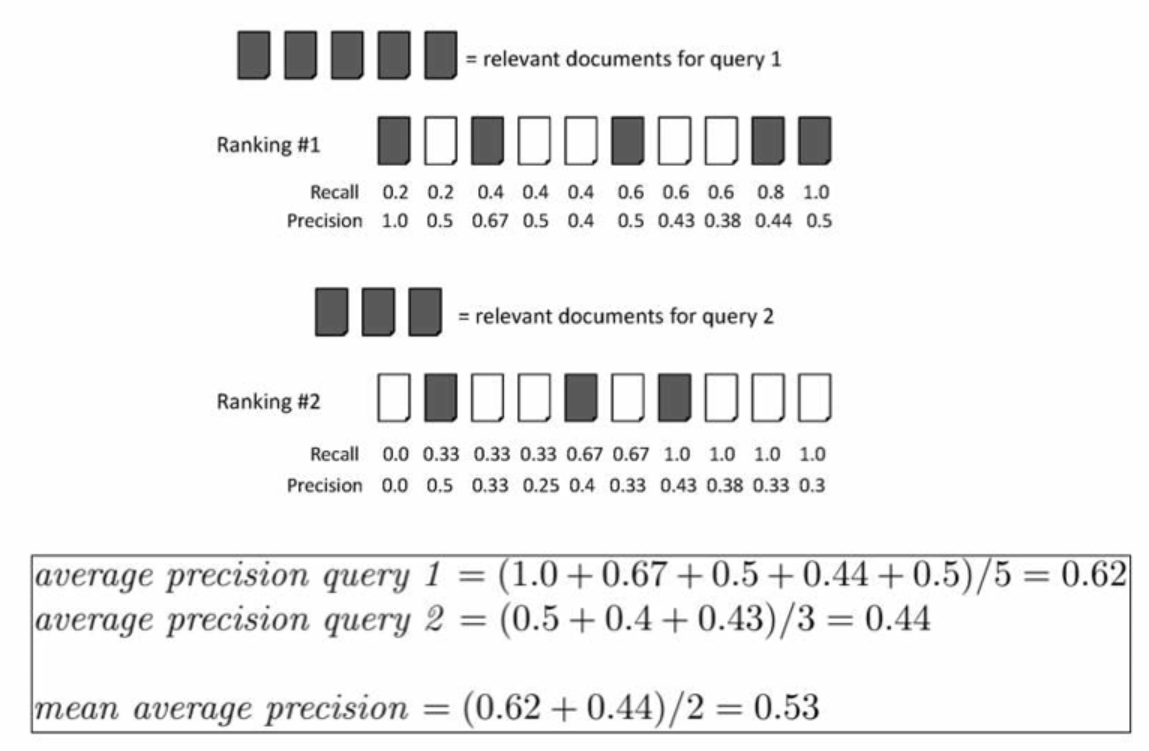
\includegraphics[width=6.5cm]{img/map.png} 
\end{wrapfigure} 
\textbf{average precision of a query is:} $1/n\sum_{i=1}^n p(i)$ \\
n = number of relevant documents retrieved.\\
p(i) = precision of relevant document i.\\
\textbf{mean average precision:}
\end{frame}


\section{Dataset/Compression}

\begin{frame}{Table of Contents}
        \tableofcontents[currentsection,currentsubsection]
\end{frame}

\subsection{Dataset}
\begin{frame}{Dataset}
\begin{block} {Oxford Buildings Dataset}
	\begin{itemize}
		\item 5062 images
		\item compressed loss-less or with minimal loss in JPEG
		\item collected from Flickr by searching for particular Oxford landmarks
		\item manually annotated to generate ground truth for 11 different landmarks
		\item 5 queries per landmark
		\item total of 55 queries
	\end{itemize}
\end{block}
	Random sampled subsets to limit compression and benchmark speed!
\end{frame}

\begin{frame} {Estimate Compression Ratio}
Because the dataset we used was JPEG compressed we first estimated the compression ratio.
			\begin{block}{t}	
				$s$ : avg size = 391.659 bytes.\\
				$p$ :  avg pixels = 765.969 pixel.\\
				$bpp$ : byte per pixel = 3.\\
				$r$ : avg raw size = $p*bpp$ = 2297908.\\
				$e$ : estimated ratio = $r/s = 5.867$.
			\end{block}	
			So we have a ratio smaller 6.
\end{frame}

\begin{frame}{Queries}
	The query consists of a reference image and 4 query sets:
	\begin{itemize}
		\item [good] A nice, clear picture of the object
		\item [ok] More than 25\% of the object is clearly visible.
		\item [junk] Junk Less than 25\% of the object is visible, or there are very high levels of occlusion or distortion.
		\item [bad]  Object not present
	\end{itemize}
	\begin{tabular}{ll}
		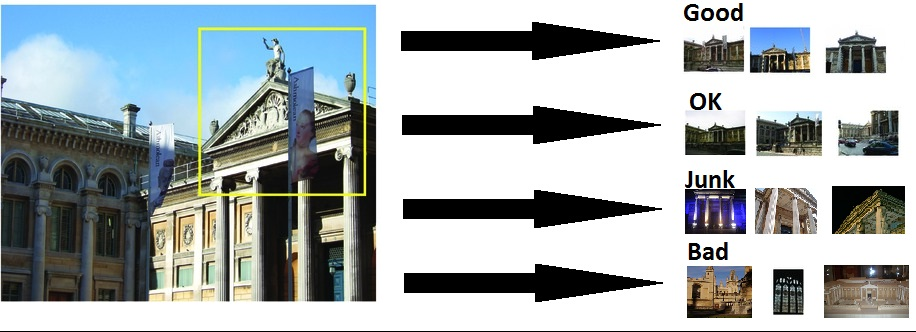
\includegraphics[width=0.7\textwidth]{img/query.jpg}
	\end{tabular}
	now similarity between these image is measured
\end{frame}


\begin{frame}{Mean Average Precision add}
VlBenchmark uses a slightly different scheme, but the calculation stays the same.
	\begin{block}{How use the four query classes}
		\begin{itemize}
			\item good and ok images are relevant
			\item junk will be ignored
			\item bad will count as wrong
		\end{itemize}
	\end{block}
Junk images do not influence precision or recall!
\end{frame}

\begin{frame} {Generic Local Feature Extractor}
The Ranking in VlBenchmark is done using Local Feature Extractors. The purpose of the Feature Extractor is to calculate frames and corresponding descriptors from the image data.
	\begin{block}{Local Feature Frames}
		\begin{itemize}
			\item search image for interest points
			\item define a frame for that point(points,circles,elipses)
		\end{itemize}
	\end{block}	 
	\begin{block}{Descriptor}
		\begin{itemize}
			\item compute descriptor using the image data defined by the sframe
			\item every descriptor is a vector of same dimension
		\end{itemize}
	\end{block}
	So we got n frames and n descriptors
\end{frame}

\begin{frame} {Retrieval System}
	\begin{block}{Ranking}
		\begin{itemize}
			\item calculate KNN for the every reference descriptor
			\item vote with descriptor distance for the image
			\item normalize
			\item sort images after voting
		\end{itemize}
	\end{block}
		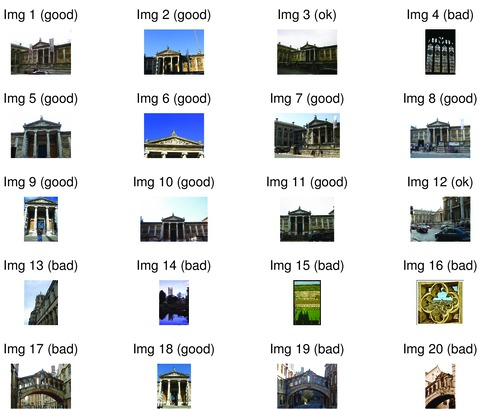
\includegraphics[width=0.5\textwidth]{img/retrieved.jpg}
\end{frame}


\subsection{Compression}
\begin{frame}{Compression}
\begin{tabular}{|l||c|c|c|}
\hline
& jpg & jxr & jp2 \\
\hline
min avg size in bytes & 13229 & 1756 & 511 \\
\hline
\end{tabular}
\begin{figure}
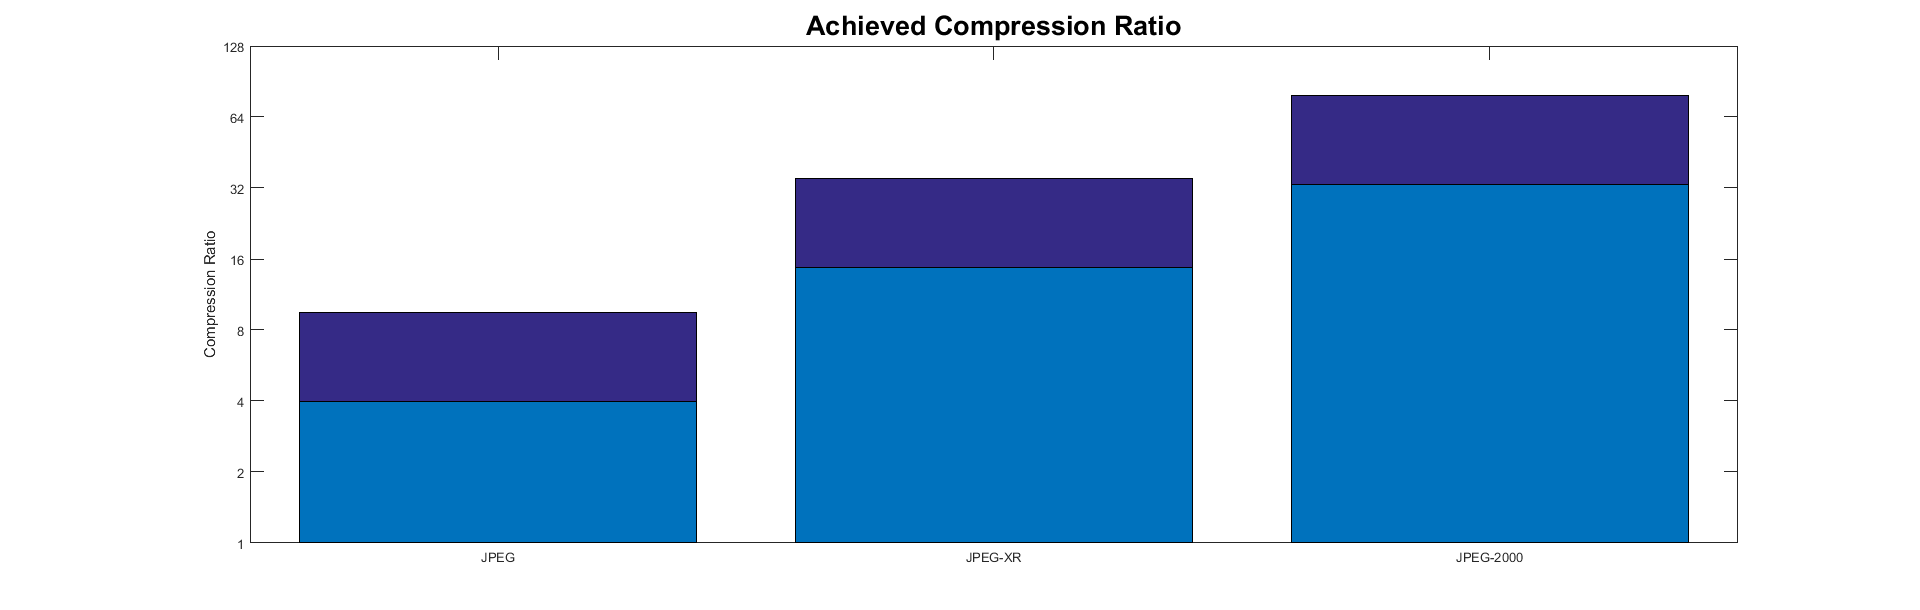
\includegraphics[width=1\textwidth]{img/ratio.png}
		\caption{light is ratio compared to jpg, dark compared to avg. raw size}
\end{figure}
\end{frame}

\begin{frame}{Sample}
	\begin{figure}
		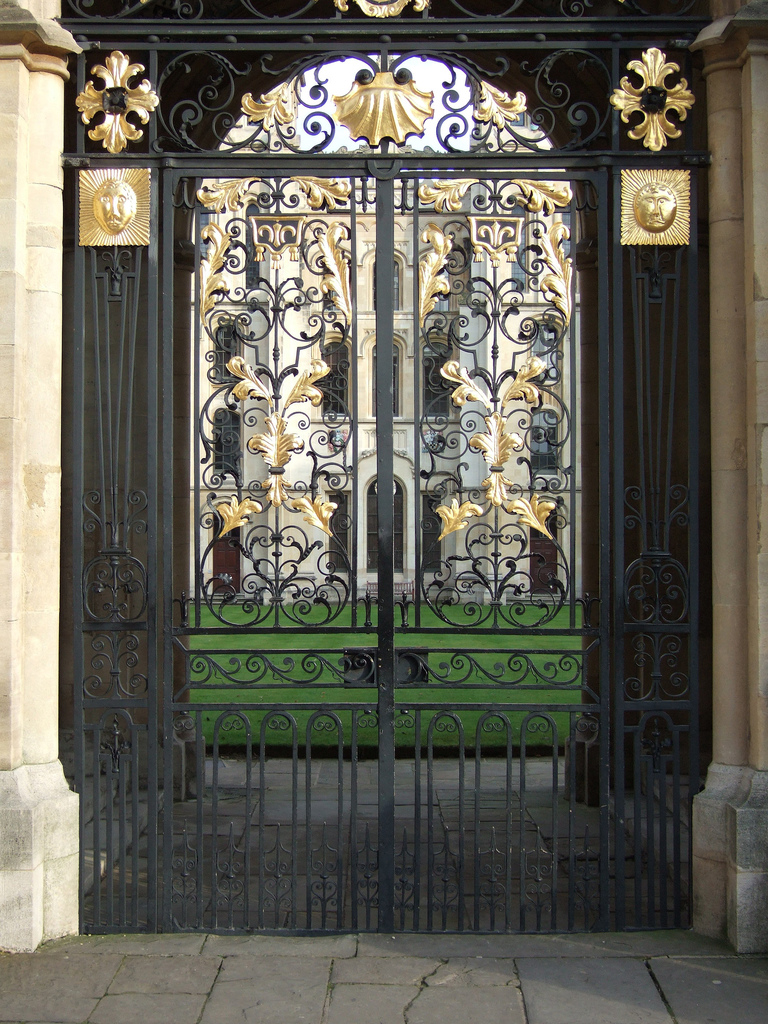
\includegraphics[width=0.5\textwidth]{img/jpg_100.jpg}
	\end{figure}
\end{frame}



\begin{frame}{Comparison}
	\begin{figure}
		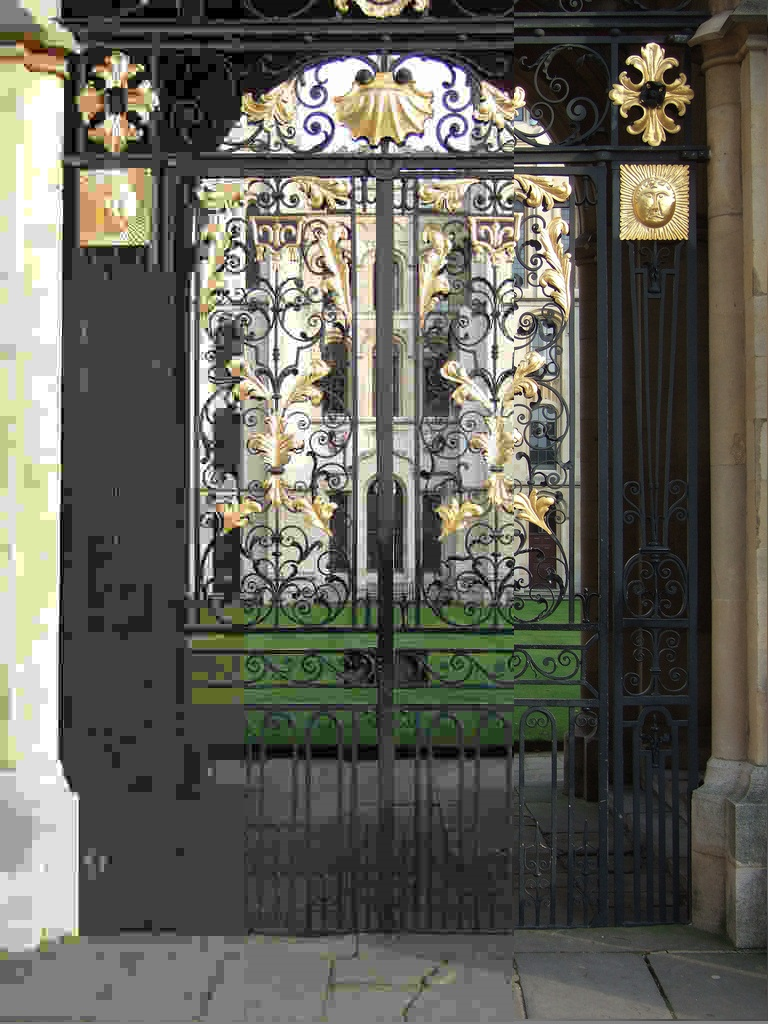
\includegraphics[width=0.35\textwidth]{img/jpg.jpg}
		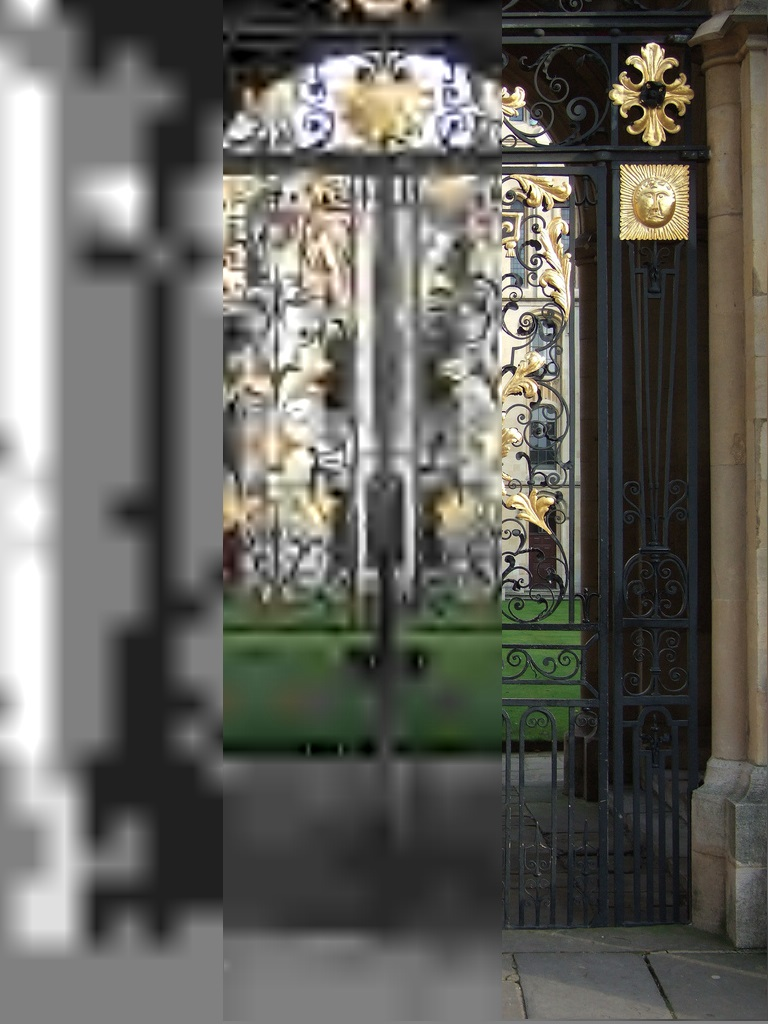
\includegraphics[width=0.35\textwidth]{img/jp2.jpg}
		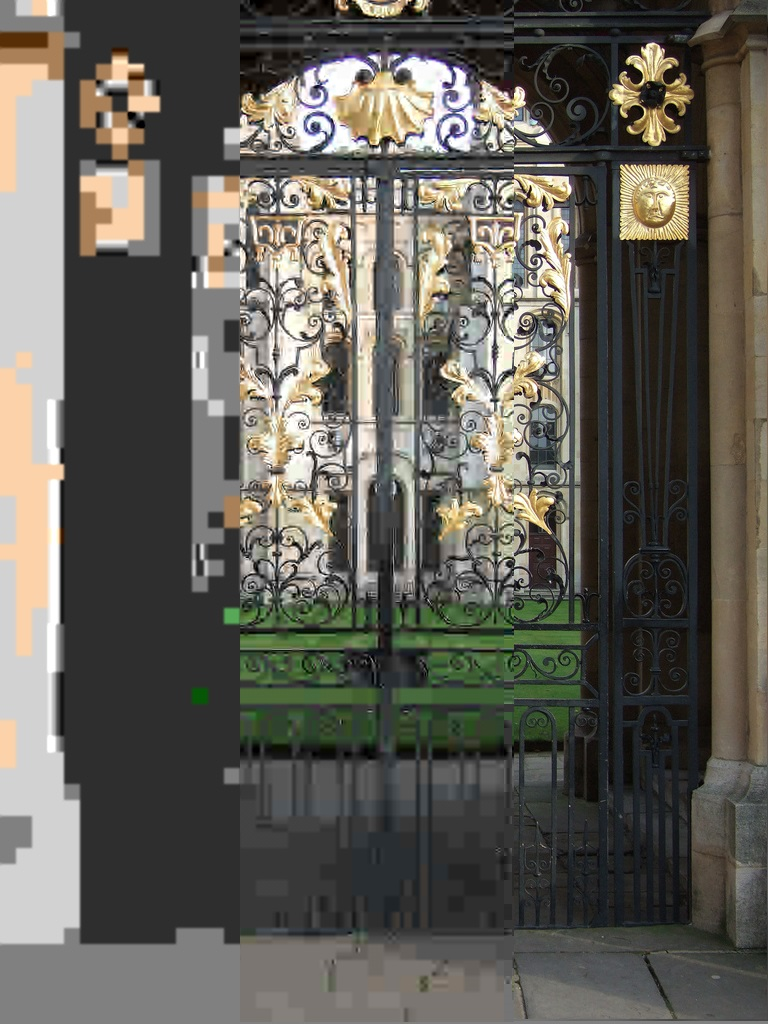
\includegraphics[width=0.35\textwidth]{img/jxr.jpg}
	\end{figure}
\end{frame}

\begin{frame}
	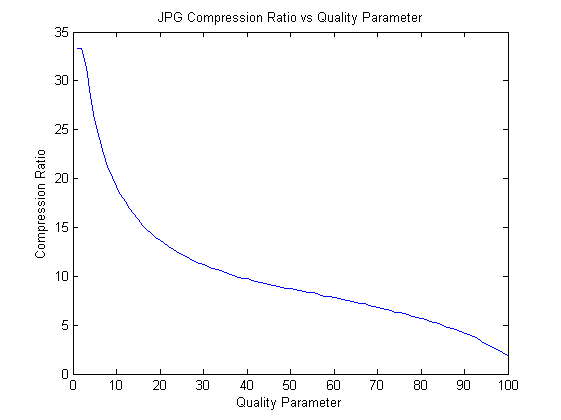
\includegraphics[width=0.8\textwidth]{img/jpg-ratio.png}
\end{frame}

\section{Feature Detectors}

\begin{frame}{Table of Contents}
        \tableofcontents[currentsection,currentsubsection]
\end{frame}

\begin{frame}{FeatureDetectors}
	\begin{itemize}
		\item vlfeat
		\begin{itemize}
			\item SIFT
			\item PHOW(DSIFT)
		\end{itemize}
		\item opencv
		\begin{itemize}
			\item SURF
			\item ORB
		\end{itemize}
	\end{itemize}
\end{frame}

\section{Results}
\begin{frame}{Results}
	\begin{itemize}
		\item plot of mAP over image file size
		\item plot query precision
		\item plot prc
	\end{itemize}
\end{frame}

\subsection{JPEG-2000}
\begin{frame} {MAP over Ratio}
	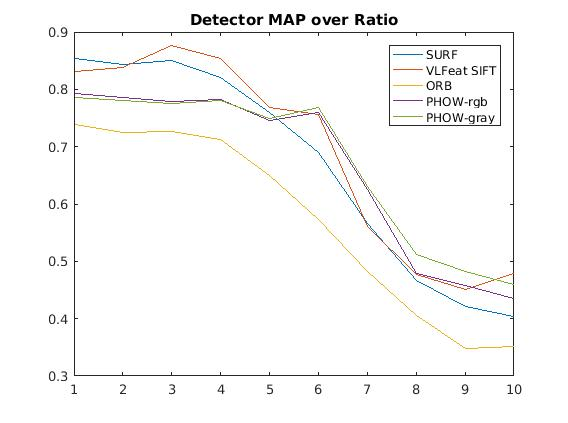
\includegraphics[width=0.8\textwidth]{img/jp2_map.jpg}
\end{frame}

\begin{frame} {Query AP over Ratio}
	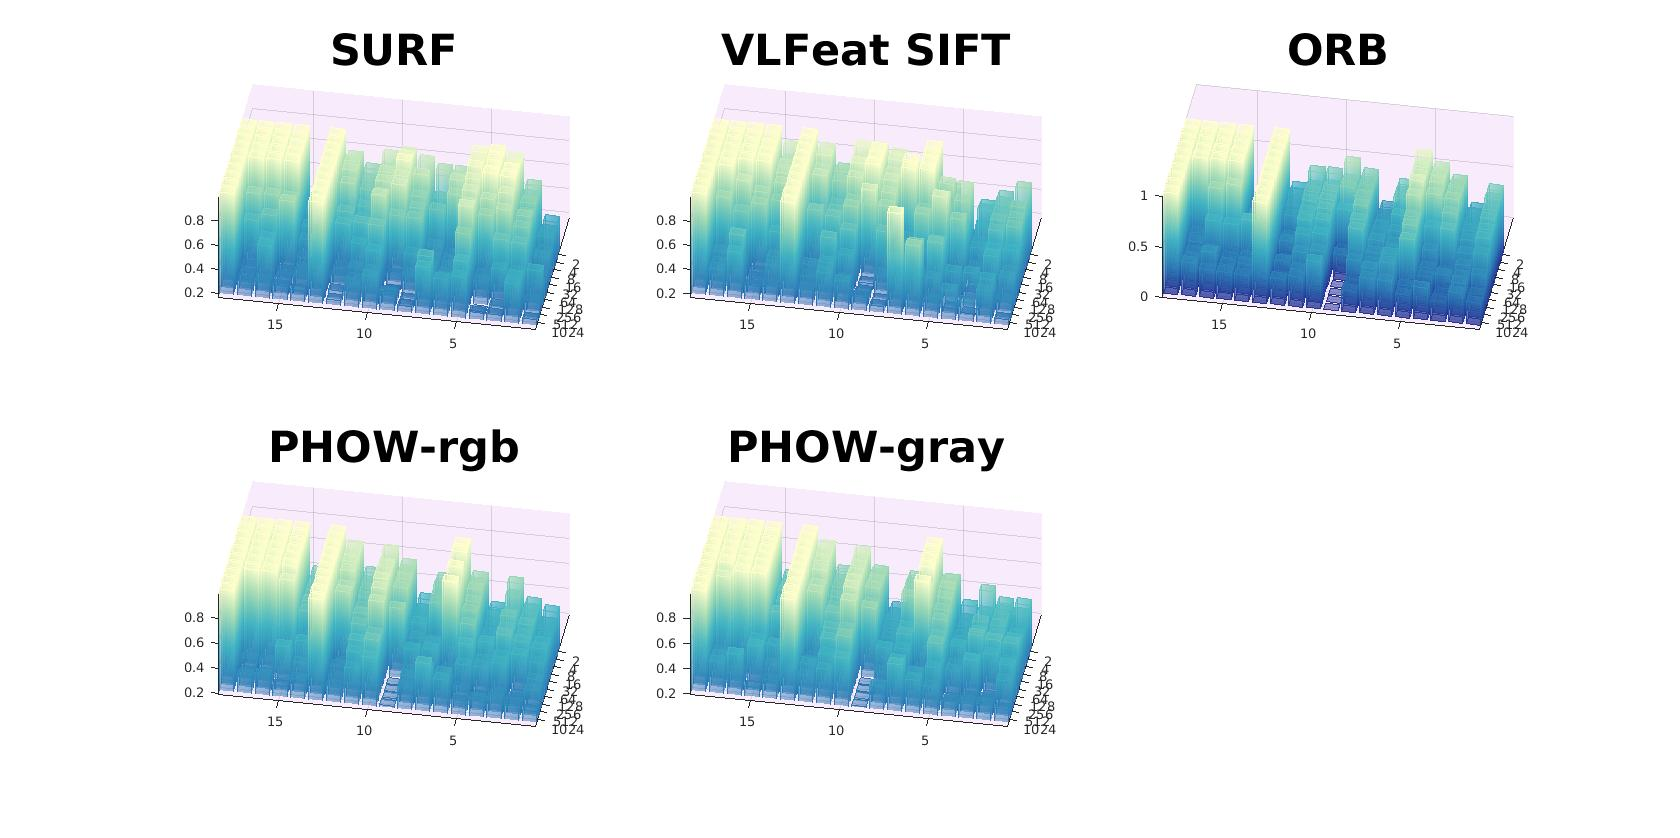
\includegraphics[width=1\textwidth]{img/jp2_queryAp.jpg}
\end{frame}

\begin{frame} {PRC over Ratio}
	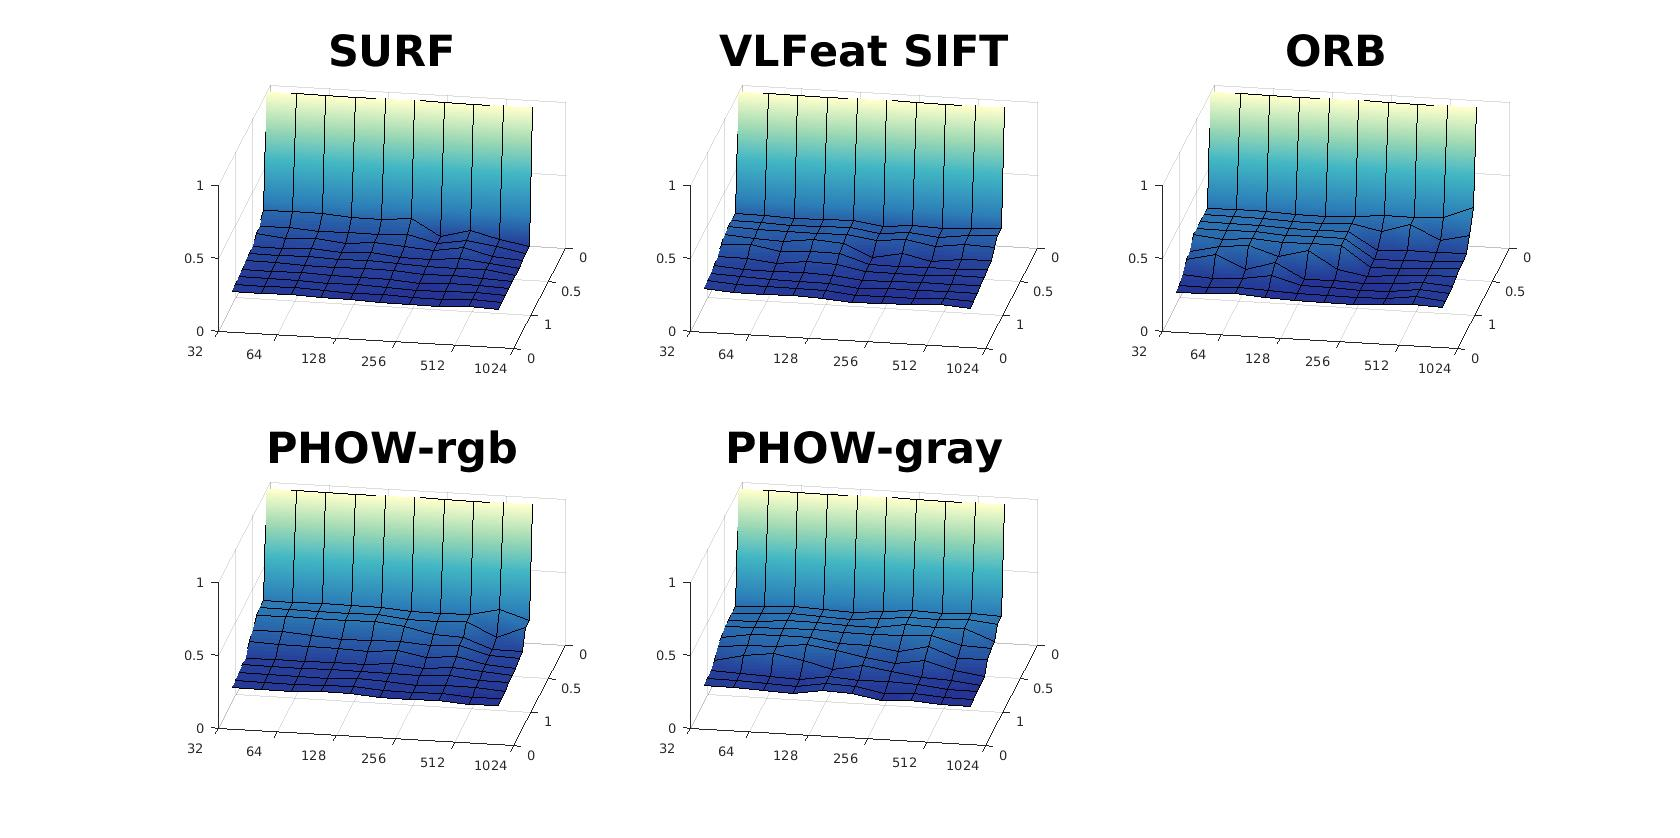
\includegraphics[width=1\textwidth]{img/jp2_prc.jpg}
\end{frame}

\subsection{JPEG-XR}
\begin{frame} {MAP over Ratio}
	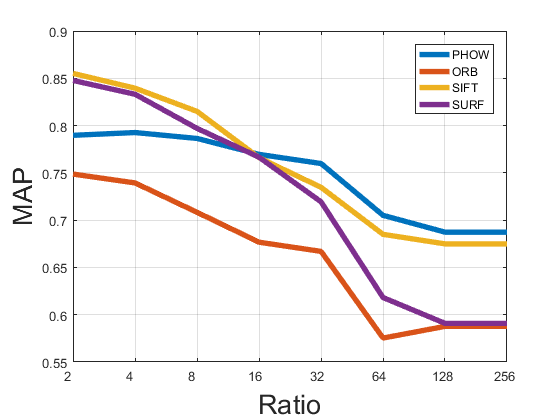
\includegraphics[width=0.8\textwidth]{img/jxr_map.png}
\end{frame}

\begin{frame} {Query AP over Ratio}
	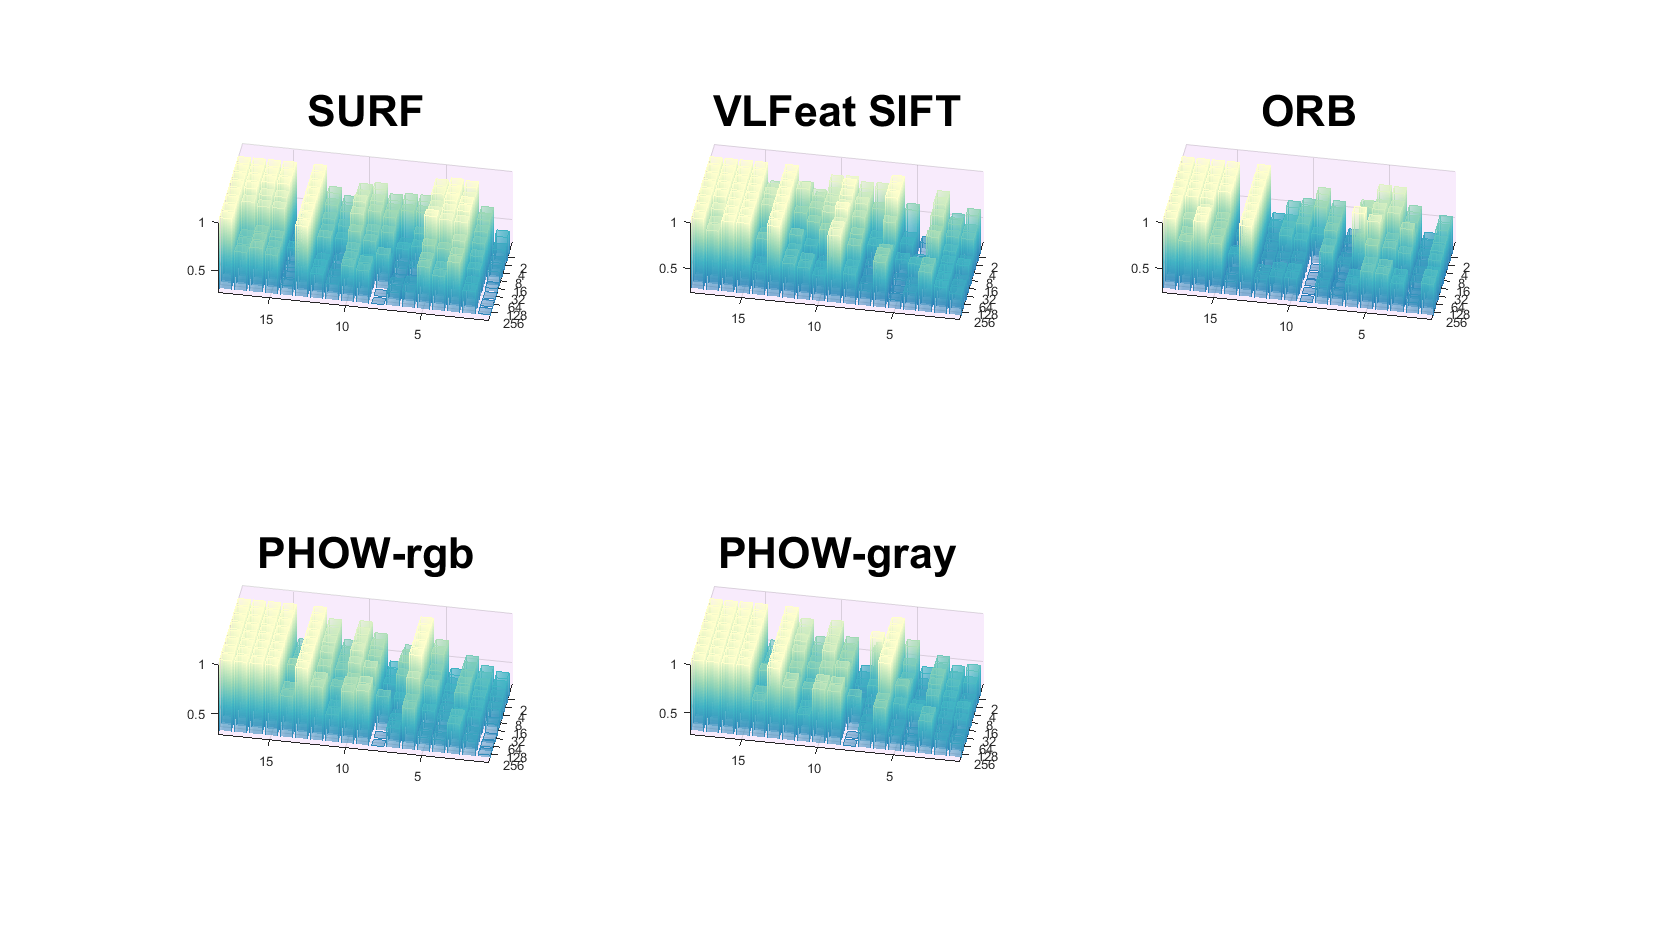
\includegraphics[width=1\textwidth]{img/jxr_queryAp.png}
\end{frame}

\begin{frame} {PRC over Ratio}
	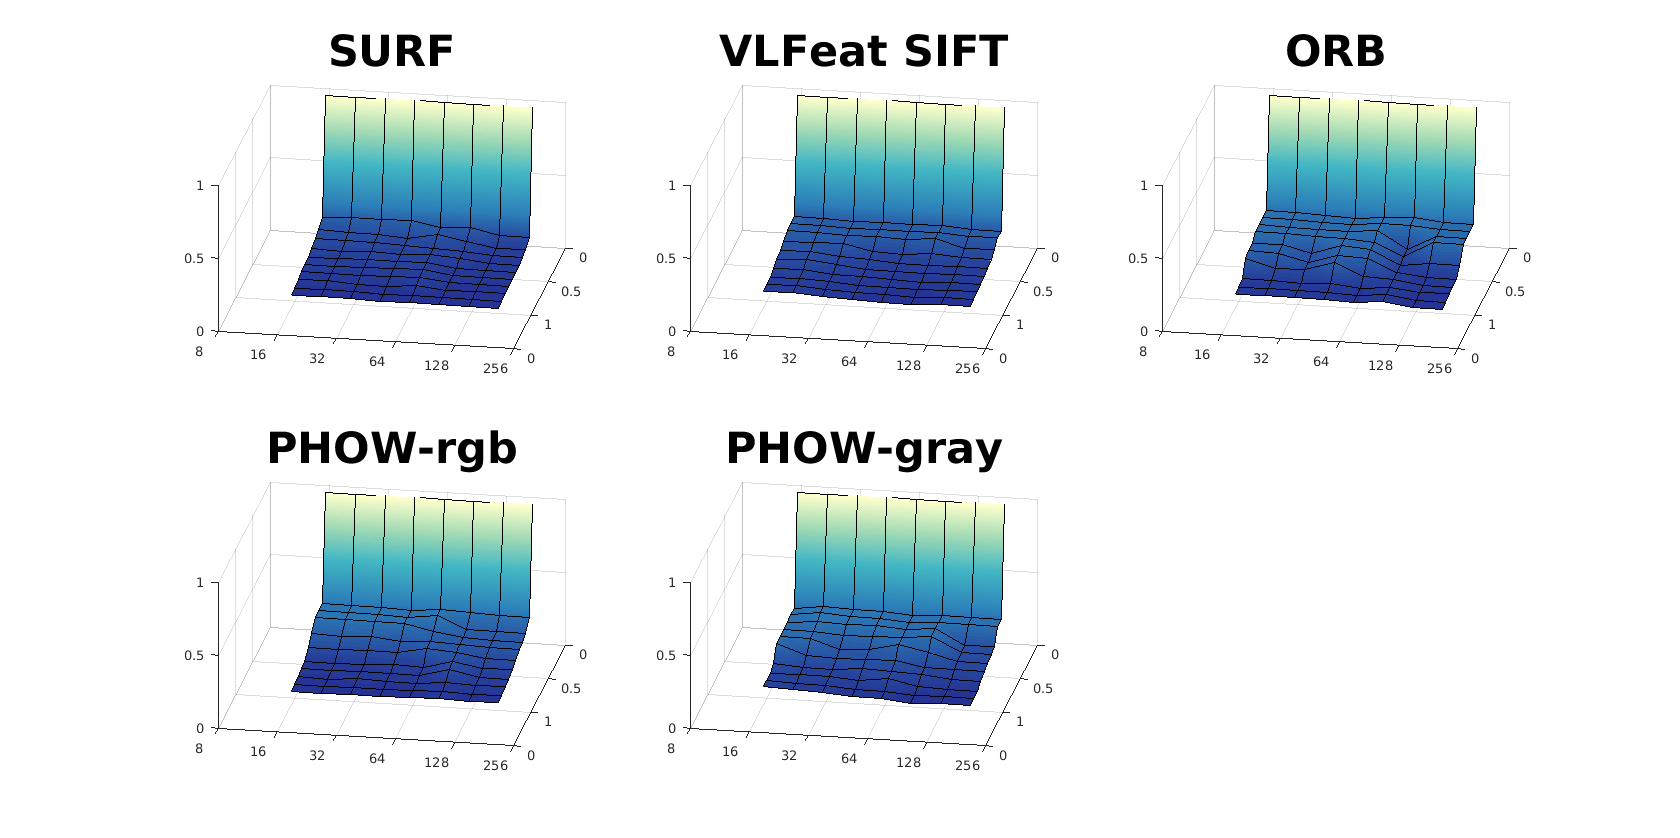
\includegraphics[width=1\textwidth]{img/jxr_prc.png}
\end{frame}

\subsection{JPEG}
\begin{frame} {MAP over Ratio}
	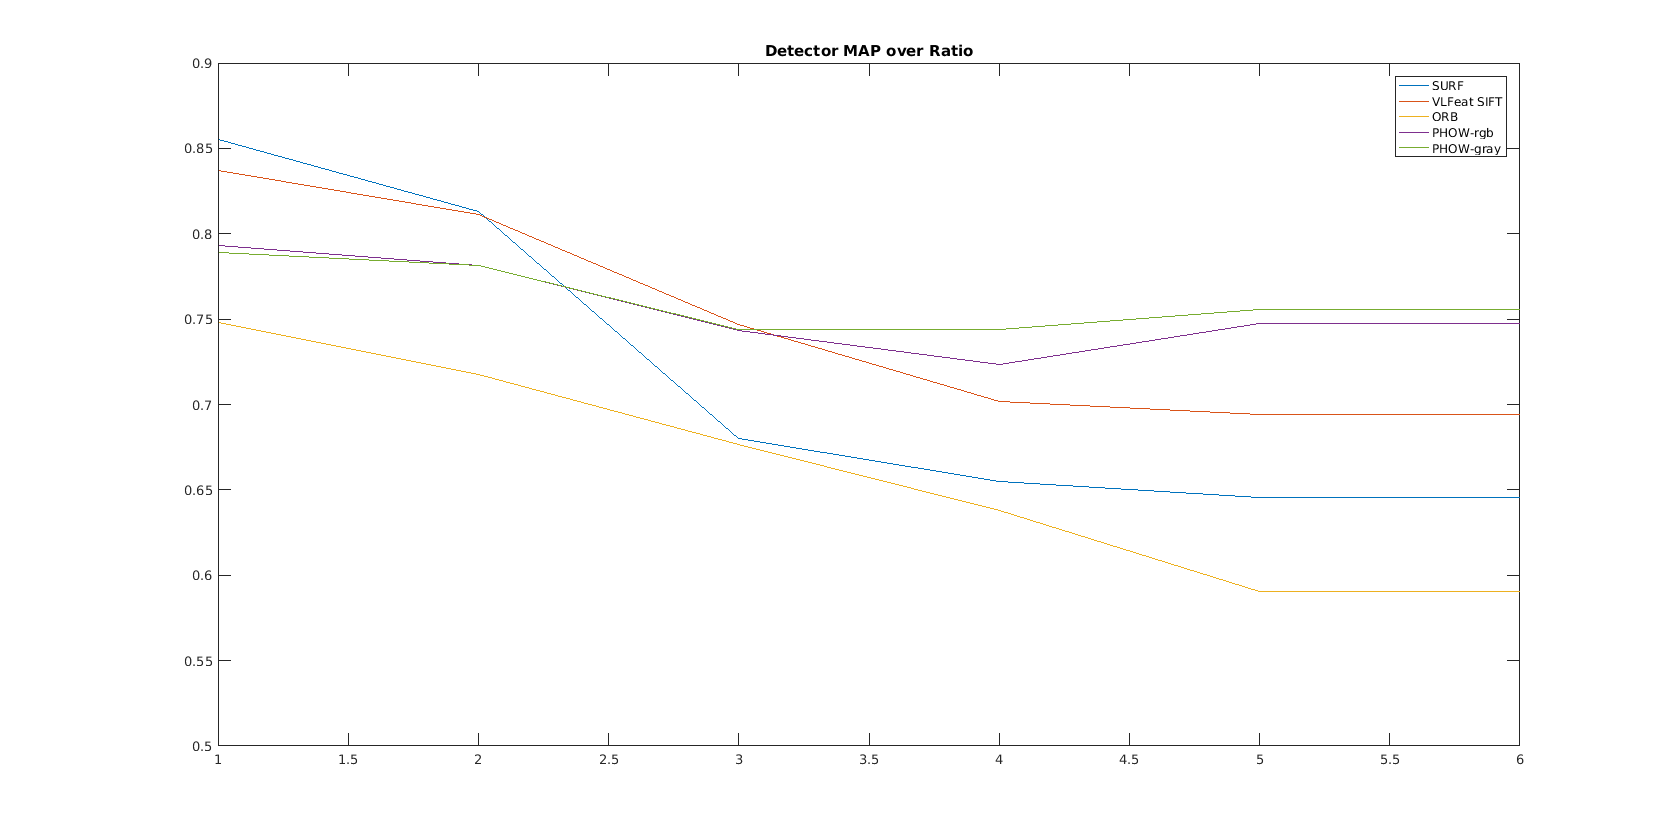
\includegraphics[width=0.8\textwidth]{img/jpg_map.png}
\end{frame}

\begin{frame} {Query AP over Ratio}
	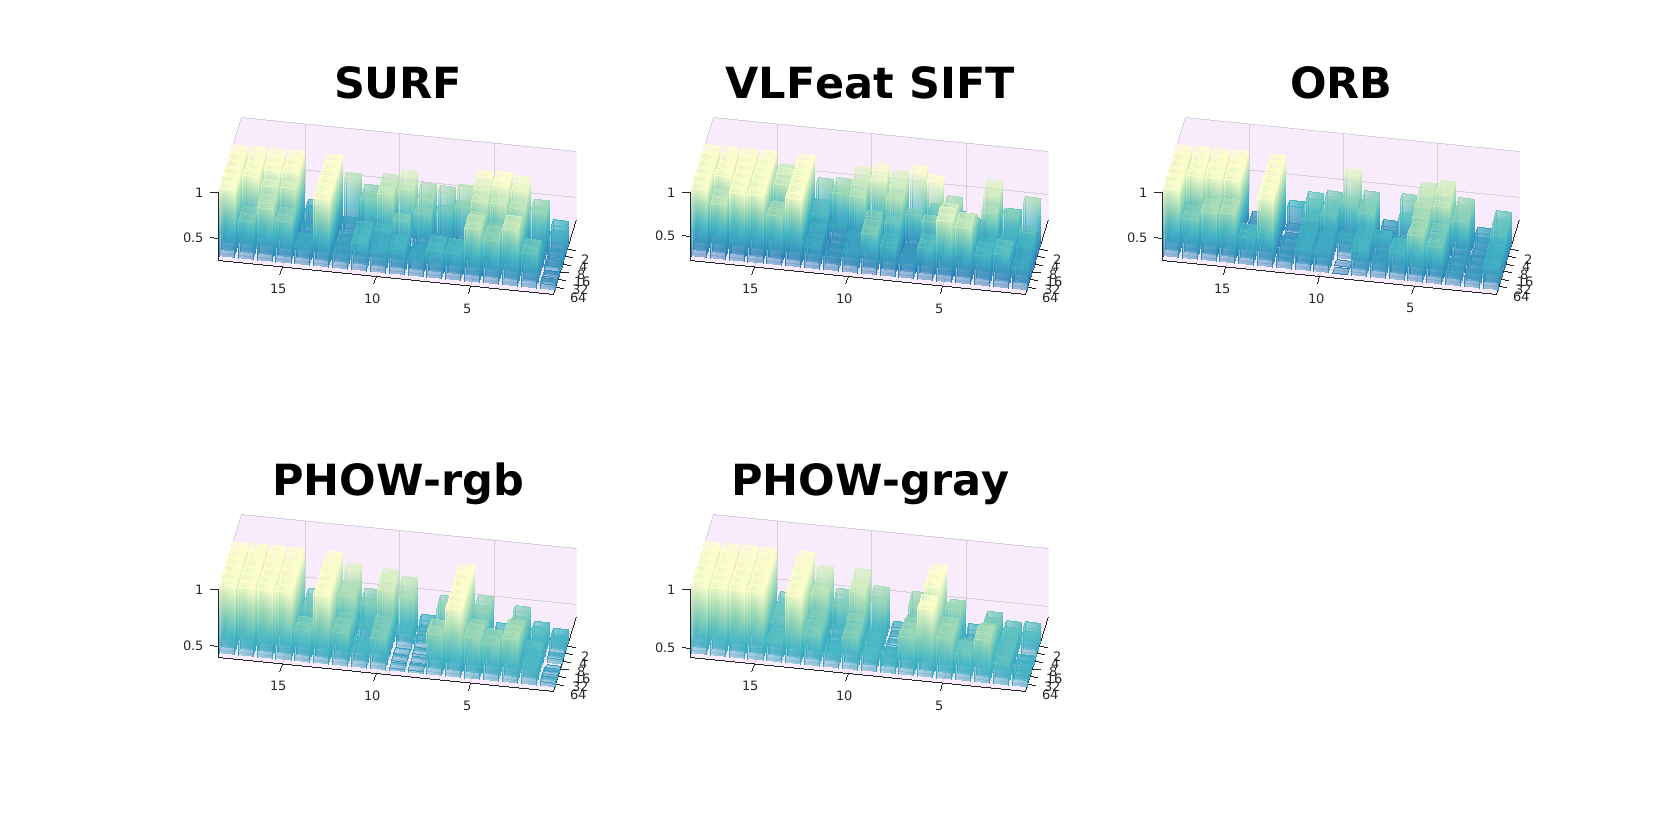
\includegraphics[width=1\textwidth]{img/jpg_queryAp.png}
\end{frame}

\begin{frame} {PRC over Ratio}
	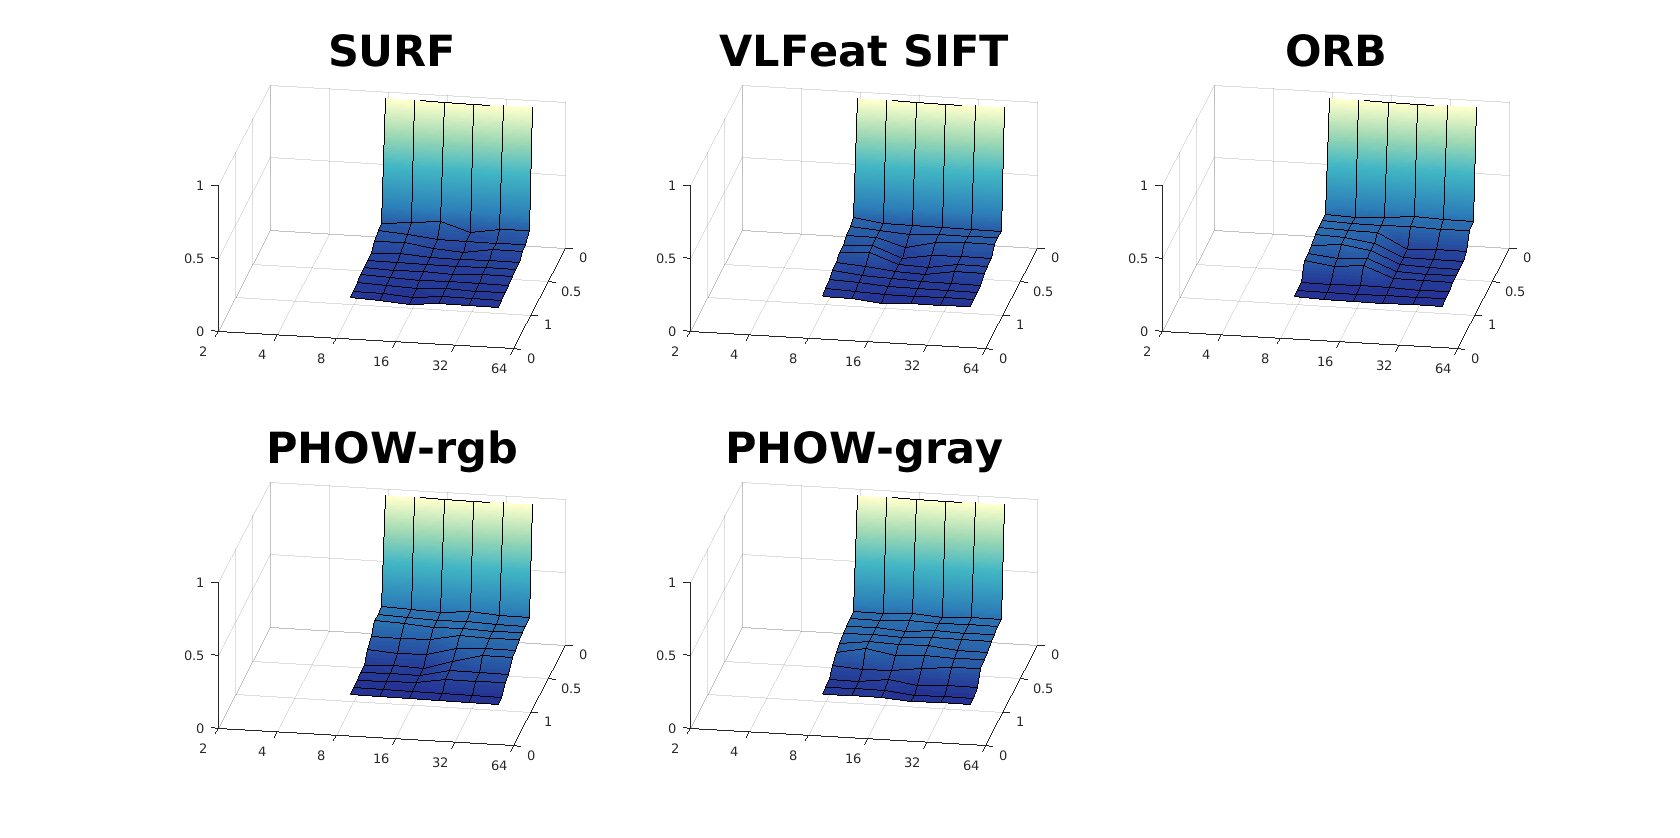
\includegraphics[width=1\textwidth]{img/jpg_prc.png}
\end{frame}

\end{document}
